\documentclass[14pt,aspectratio=169]{beamer}

% Assets
\usepackage[czech]{babel}				% Jazyk
\usepackage[a-2u]{pdfx}					% Kopírování z pdfka
\usepackage{tikz}						% Schémata automatů
\usepackage{csquotes}					% české uvozovky
\usepackage{enumerate}					% enumerate environment
\usepackage{indentfirst}
\usepackage{mathtools}
\usepackage{pifont}
\usepackage{xcolor}
\usepackage{enumitem,xcolor}
\usepackage{amsmath}
\usepackage[utf8]{inputenc}

\usepackage{listings}                   % Úryvky z kódu (C#)
\lstset{language=[Sharp]C, frame=lr}
% Beamer theme
\usetheme{Boadilla}
\setbeamertemplate{frame numbering}[fraction]
\usecolortheme[named=black]{structure}
\setbeamertemplate{navigation symbols}{}
\setbeamerfont{title}{series=\bfseries,parent=structure}
\setbeamerfont{frametitle}{series=\bfseries,parent=structure}
\usefonttheme[onlymath]{serif}
\urlstyle{same}

% Dark theme
\setbeamercolor{frametitle}{fg=white}
\setbeamercolor{title}{fg=white}
\setbeamercolor{background canvas}{bg=black}
\setbeamercolor{normal text}{fg=white}

\defbeamertemplate*{title page}{customized}[1][]
{ 
  \usebeamerfont*{title}\inserttitle\par
  \bigskip
  \usebeamerfont*{subtitle}\textit{\insertsubtitle}\par
  \bigskip \bigskip \bigskip \bigskip 
  \usebeamerfont{author}\insertauthor\par
  \usebeamerfont{institute}Kabinet \office\\\url{weber3@spsejecna.cz}\bigskip
}
% Enumerate
%\setlist[enumerate]{topsep=0pt,itemsep=-1ex,partopsep=1ex,parsep=1ex,label=(\arabic*)}

\MakeOuterQuote{"}

% Colors
\definecolor{lightblue}{HTML}{009AD4}
\definecolor{darkgreen}{HTML}{0D7103}
\definecolor{lightgreen}{HTML}{68FF00}
\definecolor{darkred}{HTML}{AF0B0B}
\definecolor{lightred}{HTML}{FF5100}
\definecolor{orange}{HTML}{FFE000}
\definecolor{codeblue}{HTML}{FF0055}
\definecolor{codegreen}{rgb}{0,0.6,0}
\definecolor{codegray}{rgb}{0.5,0.5,0.5}
\definecolor{codebeige}{HTML}{D4A000}
\definecolor{backcolour}{rgb}{0.95,0.95,0.92}

\newcommand{\markred}[1]{\textcolor{lightred}{#1}}
\newcommand{\markgreen}[1]{\textcolor{lightgreen}{#1}}
\newcommand{\markorange}[1]{\textcolor{orange}{#1}}
\newcommand{\markblue}[1]{\textcolor{lightblue}{#1}}

% Inline images
\newcommand{\inlineimgscale}{1.1}

% X and check mark
\newcommand{\cmark}{\markgreen{\ding{51}}}
\newcommand{\xmark}{\markred{\ding{55}}}

% Redefinions
\renewcommand{\implies}{\Rightarrow}
\renewcommand{\impliedby}{\Leftarrow}

% Math
\newcommand{\R}{\mathbb{R}}
\newcommand{\C}{\mathbb{C}}
\newcommand{\N}{\mathbb{N}}
\newcommand{\Z}{\mathbb{Z}}
\newcommand{\Q}{\mathbb{Q}}

% Code
\lstdefinestyle{clang}{
    basicstyle=\small\ttfamily\color{white},
    language=C,
    keywordstyle=\color{codeblue},
    commentstyle=\color{codegreen},
    numberstyle=\tiny\color{codegray},
    stringstyle=\color{codebeige},
    breakatwhitespace=false,
    breaklines=true,
    captionpos=b,
    keepspaces=true,
    numbersep=5pt,
    showspaces=false,
    showstringspaces=false,
    showtabs=false,
    morekeywords={void,int,double,float,unsigned,if,else,\#include}
    tabsize=0.5
}
\lstset{escapeinside={(*}{*)},style=clang}

\newcommand{\hlcode}[1]{\colorbox{red}{#1}}

% Title page
\title{Řetězce v C}
\subtitle{Informační a komunikační technologie}
\author{David Weber}
\def\office{K13}
\def\email{weber3@spsejecna.cz}

\begin{document}

    % Itemize
    \setlist[itemize]{label=\textcolor{white}{\textbullet}}

    % Slides
    \begin{frame}
        \titlepage
    \end{frame}

    \begin{frame}[t]{Co dnes probereme}
        \begin{itemize}
            \item Datový typ \markblue{\texttt{char}}
            \item Práce s řetězci
            \item Užitečné funkce (knihovna \texttt{string.h})
        \end{itemize}
    \end{frame}

    \begin{frame}[t,fragile]{Zpět k datovým typům\dots}
        \begin{itemize}
            \item Zatím jsme pracovali s číselnými proměnnými $\implies$ \markblue{\texttt{int}}, \markblue{\texttt{float}}, \markblue{\texttt{double}}.
            \item Avšak např. u funkcí \texttt{printf} a \texttt{scanf} jsme jako parametr předávali ``text''.
            \item $\implies$ To jsou tzv. \textbf{řetězce} (angl. \emph{string}).
            \begin{lstlisting}
printf("Hello World!");
            \end{lstlisting}
            \item Řetězce se skládají z tzv. \textbf{znaků} (angl. \emph{char}).
        \end{itemize}
    \end{frame}

    \begin{frame}[t,fragile]{Znaky \textrm{I}}
        \begin{itemize}
            \item Znaky jsou ukládány do datového typu \markblue{\texttt{char}}
            \begin{itemize}
                \item 8 bitů
            \end{itemize}
            \item Znaky vždy uvádíme mezi apostrofy, např. \texttt{'t'}.
            \begin{lstlisting}
char znak = 'c';
            \end{lstlisting}
            \item Pracujeme s nimi stejně, jako s ostatními datovými typy, tzn. lze do nich \emph{přiřazovat}, porovnávat je pomocí \texttt{==}, \dots
            \item Pro výpis a načtení znaku používáme formátovou specifikaci \texttt{\%c}.
            \begin{lstlisting}
scanf("%c", &znak);
printf("Ulozeny znak: %c", znak);
            \end{lstlisting}
        \end{itemize}
    \end{frame}

    \begin{frame}[t,fragile]{Znaky \textrm{II}}
        \begin{itemize}
            \item Znaky, které lze do datového typu \texttt{char} ukládat nemusí být nutně \textbf{tisknutelné}.
            \item Lze např. uložit i znak pro \emph{odřádkování}.
            \begin{lstlisting}
char newLine = '\n';
            \end{lstlisting}
            \markred{$\implies$ Pozor! Ač \texttt{\textbackslash} a \texttt{n} představují \emph{dva znaky}, dohromady reprezentují \textbf{jeden znak}!}
        \end{itemize}
    \end{frame}

    \begin{frame}[t,fragile]{Znaky \textrm{III}}
        \begin{itemize}
            \item \markred{Datový typ \texttt{char} je ve skutečnosti také číselný!}
            \item Např. příkaz
            \begin{lstlisting}
printf("%d", 'c');
            \end{lstlisting}
            vypíše do konzole číslo $99$.
            \item \emph{Proč tomu tak je?} $\implies$ Každý znak má svůj kód v tzv. tabulce \textbf{ASCII}.
        \end{itemize}
    \end{frame}

    \begin{frame}[t,fragile]{ASCII}
        \begin{itemize}
            \item ASCII $=$ \emph{American Standard for Information Interchange}
            \item Definuje znaky \emph{anglické abecedy} a jiné znaky.
            \item Každý znak má v tabulce svůj (dnes \emph{osmibotový}) kód, kterým je identifikován.
            \item Např.
            \begin{itemize}
                \item \texttt{a} $\rightarrow$ kód \markorange{$\text{\texttt{0x61}}=97$}
                \item \texttt{b} $\rightarrow$ kód \markorange{$\text{\texttt{0x62}}=98$}
                \item \texttt{c} $\rightarrow$ kód \markorange{$\text{\texttt{0x63}}=99$}
                \item \texttt{M} $\rightarrow$ kód \markorange{$\text{\texttt{0x4D}}=77$}
                \item \texttt{M} $\rightarrow$ kód \markorange{$\text{\texttt{0x4E}}=78$}
                \item \dots
            \end{itemize}
        \end{itemize}
    \end{frame}

    \begin{frame}[t]{Kódování v ASCII}
        \begin{itemize}
            \item Každý znak je reprezentován $8$ bity $=$ \textbf{$2$ číslice v hexadecimální soustavě}.
            \item Každá číslice určuje \textbf{řádek}, resp. \textbf{sloupec} v tabulce.
            \item $\implies$ V proměnné datového typu \markblue{\texttt{char}} je tak uložena \textbf{ASCII hodnota daného znaku}.
            \item Přehled všech znaků v ASCII např. \href{https://www.asciitable.com/}{\underline{zde}}.
        \end{itemize}
    \end{frame}

    \begin{frame}{Tabulka ASCII}
        Prvních $127$ znaků tabulky ASCII (obrázek převzat z \href{https://cs.wikipedia.org/wiki/ASCII}{\underline{Wikipedie}}).
        \begin{figure}
            \centering
            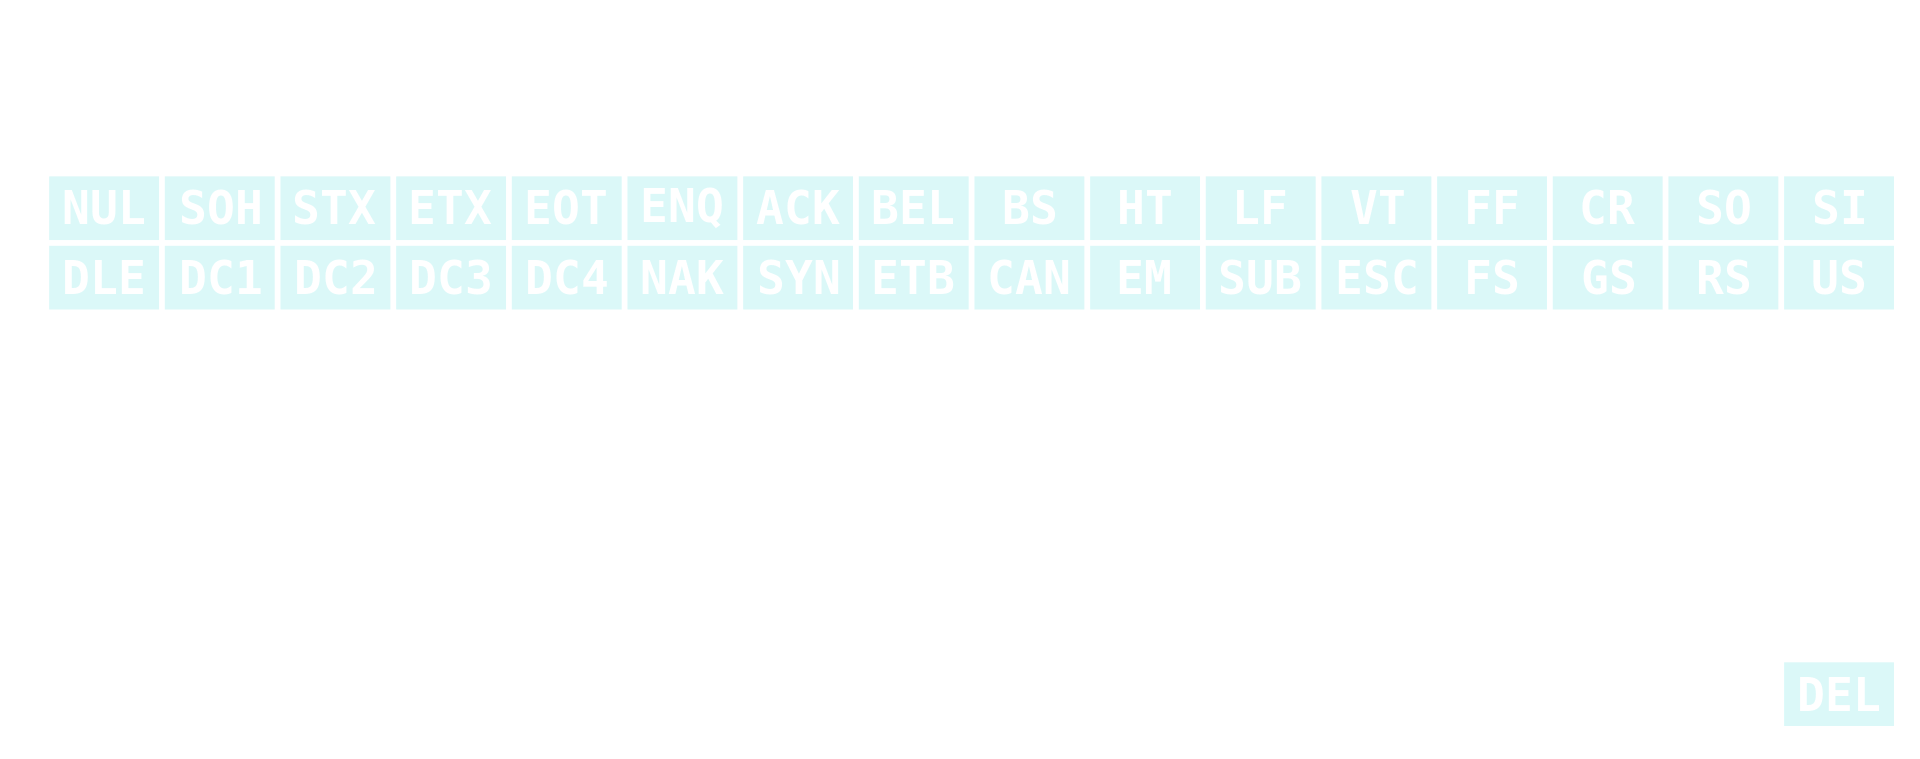
\includegraphics[scale=.22]{images/ASCII_Code_Chart.png}
        \end{figure}
    \end{frame}

    \begin{frame}[t,fragile]{Řetězce \textrm{I}}
        \begin{itemize}
            \item Řetězec představuje jistou \textbf{posloupnost znaků}.
            \item V jazyce C jsou reprezentovány jako \textbf{pole znaků}.
            \begin{itemize}
                \item \markorange{$\implies$} Jako datový typ uvádíme tedy \texttt{\markblue{char}[]}.
                \item Každý retězec je zakončen znakem tzv. \emph{nulovým znakem} \texttt{'\textbackslash0'} reprezentující konec slova.
            \end{itemize}
            \item Řetězec lze inicializovat přímo jako pole
            \begin{lstlisting}
char pozdrav[] = { 'A', 'h', 'o', 'j', '\0' };
            \end{lstlisting}
            \markred{$\implies$ Celkem nepraktické!}
        \end{itemize}
    \end{frame}

    \begin{frame}[t,fragile]{Řetězce \textrm{II}}
        \begin{itemize}
            \item Lepší znaky daného řetězce uvést do uvozovek, tj. \texttt{\textquotedblleft\dots\textquotedblright}.
            \begin{lstlisting}
char pozdrav[] = "Ahoj";
            \end{lstlisting}
            \item Znak \texttt{\textbackslash0} nemusíme uvádět $\implies$ je doplněn automaticky.
            \item Pro výpis používáme formátovou specifikaci \texttt{\%s}.
            \begin{lstlisting}
printf("%s", pozdrav);
            \end{lstlisting}
        \end{itemize}
    \end{frame}

    \begin{frame}[t,fragile]{Řetězce \textrm{III}}
        \begin{itemize}
            \item Řetězce (stringy) jsou pole znaků $\implies$ lze s nimi manipulovat pomocí indexů.
            \item Např. program
            \begin{lstlisting}
char pozdrav[] = "Ahoj";
pozdrav[1] = 't';
printf("%s", pozdrav)
            \end{lstlisting}
            vypíše slovo \texttt{Atoj}.
        \end{itemize}
    \end{frame}

    \begin{frame}[t,fragile]{Knihovna \texttt{string.h}}
        \begin{itemize}
            \item Pro práci s řetězci se nám bude hodit knihovna \texttt{string.h}
            \item Některé užitečné funkce:
            \begin{itemize}
                \item \markorange{\texttt{strlen()}} $\rightarrow$ vrací délku řetězce (počet znaků)
                \item \markorange{\texttt{strcat()}} $\rightarrow$ spojí dvojici řetězců do jednoho.
                \item \markorange{\texttt{strcpy()}} $\rightarrow$ zkopíruje obsah jednoho řetězce do druhého.
                \item \markorange{\texttt{strcmp()}} $\rightarrow$ porovná dvojici řetězců.
            \end{itemize}
        \end{itemize}
    \end{frame}

    \begin{frame}[t,fragile]{Funkce \texttt{strlen}}
        \begin{itemize}
            \item STRing LENgth
            \item Vrací délku řetězce (počet znaků).
            \item Návratový datový typ je \markblue{\texttt{int}}.
            \begin{lstlisting}
char alphabet[] = "ABCDEFGHIJKLMNOPQRSTUVWXYZ";
printf("%d", strlen(alphabet));   // 26
            \end{lstlisting}
        \end{itemize}
    \end{frame}

    \begin{frame}[t,fragile]{Funkce \texttt{strcat}}
        \begin{itemize}
            \item ConCATenate STRings
            \item Jako parametry přijímá \textbf{dvojici řetězců} \texttt{str1} a \texttt{str2}, které \textbf{spojí do jednoho} a \textbf{výsledek uloží do prvního}.
            \begin{lstlisting}
char str1[] = "Hello ";
char str2[] = "World!";

strcat(str1, str2);

printf("%s", str1); // Vypise "Hello World!"
            \end{lstlisting}
        \end{itemize}
    \end{frame}

    \begin{frame}[t,fragile]{Funkce \texttt{strcpy}}
        \begin{itemize}
            \item CoPY STRings
            \item Zkopíruje obsah \textbf{druhého řetězce do prvního} (tj. zde \texttt{str1} $\rightarrow$ \texttt{str2})
            \begin{lstlisting}
char str1[] = "Hello World!";
char str2[];    // Prazdny retezec

strcpy(str2, str1);

printf("%s", str2); // Vypise "Hello World!"
            \end{lstlisting}
        \end{itemize}
    \end{frame}

    \begin{frame}[t,fragile]{Funkce \texttt{strcmp}}
        \begin{itemize}
            \item CoMPare STRings
            \item Porovná dvojici řetězců, vrací hodnotu typu \markblue{\texttt{int}}
            \begin{itemize}
                \item $1=\text{řetězce jsou stejné}$,
                \item $\text{jiné číslo}=\text{řetězce jsou odlišné}$.
            \end{itemize}
            \begin{lstlisting}
char str1[] = "Hello";
char str2[] = "Hello";
char str3[] = "Hi";

printf("%d\n", strcmp(str1, str2));  // 0 (retezce jsou stejne)
printf("%d\n", strcmp(str1, str3));  // -4 (retezce nejsou stejne)
            \end{lstlisting}
        \end{itemize}
    \end{frame}

    \begin{frame}{Otázky?}
        \begin{figure}
            \centering
            
\includegraphics[scale=.4]{images/discussion_inverted.png}
        \end{figure}
    \end{frame}

\end{document}